In diesem Kapitel sei $X \neq \emptyset$ eine Menge.

\begin{definition}
    \index{$\sigma$-!Algebra}
    Sei $\fa\subseteq\mathcal{P}(X)$, $\fa$ heißt eine 
    \textbf{$\sigma$-Algebra} auf $X$, wenn gilt:
    \begin{enumerate}
        \item[($\sigma_1$)] $X\in\fa$
        \item[($\sigma_2$)] $A\in\fa \implies A^c\in\fa$
        \item[($\sigma_3$)] $(A_j)$ ist eine Folge in $\fa \implies$
                            $\bigcup A_j\in\fa$.
    \end{enumerate}
\end{definition}

\begin{beispieleX}
    \begin{enumerate}
        \item $\Set{X,\emptyset}$ und $\mathcal{P}(X)$ sind 
              $\sigma$-Algebren auf $X$.
        \item Sei $A\subseteq X$, dann ist $\Set{X,\emptyset, A, A^c}$ 
              eine $\sigma$-Algebra auf $X$.
        \item $\fa:=\Set{A\subseteq X | A \text{ abzählbar oder } A^c \text{ abzählbar}}$ 
              ist eine $\sigma$-Algebra auf $X$.
    \end{enumerate}
\end{beispieleX}

\begin{lemma}
\label{Lemma 1.1}
Sei $\fa$ eine $\sigma$-Algebra auf $X$, dann:
\begin{enumerate}
\item $\emptyset\in\fa$
\item Ist $(A_j)$ eine Folge in $\fa$, so ist $\bigcap A_j\in\fa$.
\item Sind $A_1,\dots,A_n\in\fa$, so gilt:
\begin{enumerate}
\item $A_1\cup\dots\cup A_n\in\fa$
\item $A_1\cap\dots\cap A_n\in\fa$
\item $A_1\setminus A_2\in\fa$
\end{enumerate}
\end{enumerate}
\end{lemma}

\begin{beweis}
    \begin{enumerate}
    \item \folgtnach{$\sigma_2$} $\emptyset=X^c\in\fa$.
    \item $D:=\bigcap A_j$. $D^c=\bigcup A_j^c\in\fa$ (nach 
          ($\sigma_2$) und ($\sigma_3$)), also gilt auch 
          $D=(D^c)^c\in\fa$.
    \item \begin{enumerate}
            \item \folgtnach{($\sigma_3$) mit $A_{n+j}:=\emptyset$ ($j\ge 1$)} 
                  $A_1\cup\dots\cup A_n\in\fa$.
            \item \folgtnach{(2) mit $A_{n+j}:=X$ ($j\ge 1)$} 
                  $A_1\cap\dots\cap A_n\in\fa$.
            \item $A_1\setminus A_2=A_1\cap A_2^c\in\fa$
          \end{enumerate}
    \end{enumerate}
\end{beweis}

\begin{lemma}
    \label{Lemma 1.2}
    Sei $\cf \neq \emptyset$ eine Menge von $\sigma$-Algebren auf $X$. 
    Dann ist 
    \[\fa_0:=\bigcap_{\fa\in\cf}\fa\]
    eine $\sigma$-Algebra auf $X$.
\end{lemma}

\begin{beweis}
    \begin{enumerate}
        \item[($\sigma_1$)] $\forall\fa\in\cf:X\in\fa\implies X\in\fa_0$.
        \item[($\sigma_2$)] Sei $A\in\fa_0$, dann gilt:
          \begin{align*}
            \forall\fa\in\cf:A\in\fa &\implies \forall\fa\in\cf:A^c\in\fa\\
                                     &\implies A^c\in\fa_0
          \end{align*}
        \item[($\sigma_3$)] Sei $(A_j)$ eine Folge in $\fa_0$, dann 
            ist $(A_j)$ Folge in $\fa$ für alle $\fa\in\cf$, dann gilt:
          \begin{align*}
            \forall\fa\in\cf:\bigcap A_j\in\fa \implies \bigcap A_j\in\fa_0
          \end{align*}
    \end{enumerate}
\end{beweis}

\begin{definition}
    \index{Erzeuger}
    Sei $\emptyset \neq \mathcal{E} \subseteq \mathcal{P}(X)$ und 
    $\cf:=\{\fa:\fa$ ist $\sigma$-Algebra auf $X$ mit 
    $\mathcal{E}\subseteq\fa\}$. Definiere
    \[\sigma(\mathcal{E}):=\bigcap_{\fa\in\cf}\fa\]
    \folgtnach{1.2} $\sigma(\mathcal{E})$ ist eine $\sigma$-Algebra 
    auf $X$. $\sigma(\mathcal{E})$ heißt die 
    \textbf{von $\mathcal{E}$ erzeugte $\sigma$-Algebra}. 
    $\mathcal{E}$ heißt ein \textbf{Erzeuger} von 
    $\sigma(\mathcal{E})$.
\end{definition}

\begin{lemma}
    \label{Lemma 1.3}
    Sei $\emptyset\ne\mathcal{E}\subseteq\mathcal{P}(X)$.
    \begin{enumerate}
        \item $\mathcal{E}\subseteq\sigma(\mathcal{E})$. 
              $\sigma(\mathcal{E})$ ist die "`kleinste"' 
              $\sigma$-Algebra auf $X$, die $\mathcal{E}$ enthält.
        \item Ist $\mathcal{E}$ eine $\sigma$-Algebra, so ist 
              $\sigma(\mathcal{E})=\mathcal{E}$.
        \item Ist $\mathcal{E}\subseteq\mathcal{E}'$, so ist 
              $\sigma(\mathcal{E})\subseteq\sigma(\mathcal{E}')$.
    \end{enumerate}
\end{lemma}

\begin{beweis}
    \begin{enumerate}
        \item Klar nach Definition.
        \item $\fa:=\mathcal{E}$, dann gilt 
              $\fa\subseteq\sigma(\mathcal{E})\subseteq\fa$.
        \item $\mathcal{E}\subseteq\mathcal{E}'\subseteq\sigma(\mathcal{E}')$, 
              also folgt nach Definition 
              $\sigma(\mathcal{E})\subseteq\sigma(\mathcal{E}')$.
    \end{enumerate}
\end{beweis}

\begin{beispiel}
    \begin{enumerate}
        \item Sei $A\subseteq X$ und $\mathcal{E}:=\{A\}$. Dann ist 
              $\sigma(\mathcal{E})=\{X,\emptyset,A,A^c\}$.
        \item $X:=\{1,2,3,4,5\}, \mathcal{E}:=\{\{1\},\{1,2\}\}$. 
              Dann gilt:
              \[\sigma(\mathcal{E}):=\{X,\emptyset, \{1\},\{2\},\{1,2\},\{3,4,5\},\{1,3,4,5\},\{2,3,4,5\}\}\]
    \end{enumerate}
\end{beispiel}

\begin{erinnerung}
    \index{Offenheit}\index{Abgeschlossenheit}
    Sei $d\in\mdn, X\subseteq\mdr^d$. $A\subseteq X$ heißt 
    \textbf{offen} (\textbf{abgeschlossen}) in $X$, genau dann wenn 
    ein offenes (abgeschlossenes) $G\subseteq\mdr^d$ existiert mit 
    $A=X\cap G$.\\
    Beachte: $A$ abgeschlossen in $X$ $\iff$ $X\setminus A$ offen in 
    $X$.
\end{erinnerung}

\begin{definition}
    \index{Borel!$\sigma$-Algebra}\index{$\sigma$-!Algebra, Borelsche}
    \index{Borel!Mengen}
    Sei $X\subseteq\mdr^d$.
    \begin{enumerate}
        \item $\mathcal{O}(X):=\Set{A\subseteq X | A \text{ ist offen in } X}$
        \item $\fb(X):=\sigma(\mathcal{O}(X))$ heißt 
              \textbf{Borelsche $\sigma$-Algebra} auf $X$.
        \item $\fb_d:=\fb(\mdr^d)$. Die Elemente von $\fb_d$ heißen 
              \textbf{Borelsche Mengen} oder \textbf{Borel-Mengen}.
    \end{enumerate}
\end{definition}

\begin{beispiel}
    \begin{enumerate}
        \item Sei $\emptyset \neq X\subseteq\mdr^d$. Ist $A\subseteq$ 
              $\stackrel{\hbox{offen}}{\hbox{abgeschlossen}}$
              in $X$, so ist $A\in\fb(X)$.
        \item Ist $A\subseteq\mdr^d$ 
              $\stackrel{\hbox{offen}}{\hbox{abgeschlossen}}$,
              so ist $A\in\fb_d$.
        \item Sei $d=1, A=\mdq$. $\mdq$ ist abzählbar, also 
              $\mdq=\{r_1,r_2,\dots\}$ (mit $r_i\ne r_j$ für $i\ne j$). 
              Also ist $\mdq=\bigcup \{r_j\}$. Sei nun $r\in\mdq$, 
              dann ist $B:=(-\infty,r)\cup(r,\infty)\in\fb_1$. Daraus 
              folgt $\{r_j\}\in\fb_1$, also auch $\mdq\in\fb_1$.\\
              Allgemeiner lässt sich zeigen: 
              $\mdq^d:=\{(x_1,\dots,x_n):x_j\in\mdq (j=1,\dots,n)\}\in\fb_d$.
        \item Sei $x_0 \in \mdr^d, \Set{x_0}$ ist abgeschlossen
              $\Rightarrow \Set{x_0} \in \fb$
    \end{enumerate}
\end{beispiel}

\begin{definition}
    \index{Intervall}
    \index{Halbraum}
    \begin{enumerate}
    \item Seien $I_1,\dots,I_d$ Intervalle in $\mdr$. 
          Dann heißt $I_1\times\dots\times I_d$ ein \textbf{Intervall} 
          in $\mdr^d$.
    \item Seien $a=(a_1,\dots,a_d), b=(b_1,\dots,b_d)\in\mdr^d$.
          \[a\le b:\iff a_j\le b_j \quad \forall j \in \Set{1, \dots, d}\]
    \item Seien $a,b\in\mdr^d$ und $a\le b$.
          \begin{align*}
            (a,b) &:= (a_1,b_1)\times(a_2,b_2)\times\dots\times(a_d,b_d)\\
            (a,b] &:= (a_1,b_1]\times(a_2,b_2]\times\dots\times(a_d,b_d]\\
            [a,b) &:= [a_1,b_1)\times[a_2,b_2)\times\dots\times[a_d,b_d)\\
            [a,b] &:= [a_1,b_1]\times[a_2,b_2]\times\dots\times[a_d,b_d]
        \end{align*}
        mit der Festlegung $(a,b):=(a,b]:=[a,b):=\emptyset$, falls 
        $a_j=b_j$ für ein $j\in\{1,\dots,d\}$.
    \item Für $k\in\{1,\dots,d\}$ und $\alpha\in\mdr$ definiere die 
          folgenden \textbf{Halbräume}:
          \begin{align*}
            H_k^-(\alpha) &:= \Set{(x_1,\dots,x_d)\in\mdr^d:x_k\le\alpha}\\
            H_k^+(\alpha) &:= \Set{(x_1,\dots,x_d)\in\mdr^d:x_k\ge\alpha}
          \end{align*}
    \end{enumerate}
\end{definition}

Beispiel für ein Intervall $(a_1, b_1) \times [a_2, b_2]$ und
die beiden Halbräume:\\
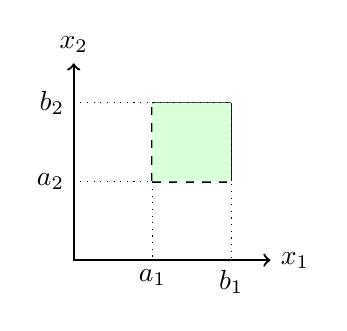
\begin{tikzpicture}
    % Draw axes
    \draw [<->,thick] (0,2.5) node (yaxis) [above] {$x_2$}
        |- (2.5,0) node (xaxis) [right] {$x_1$};

    % Draw two intersecting lines
    \draw[thick, dashed] (1,1) coordinate (a) -- (2,1) coordinate (b);
    \draw[thick, dashed] (a) -- (1,2) coordinate (d);
    \draw[thick]         (d) -- (2,2) coordinate (c);
    \draw[thick]         (b) -- (2,2);

    \fill[green!15] (a) -- (b) -- (c) -- (d) -- (a);

    % Draw lines indicating intersection with y and x axis. Here we 
    % use the perpendicular coordinate system
    \draw[dotted] (yaxis |- a) node[left] {$a_2$}
        -| (xaxis -| a) node[below] {$a_1$};

    \draw[dotted] (yaxis |- c) node[left] {$b_2$}
        -| (xaxis -| c) node[below] {$b_1$};
\end{tikzpicture}
\begin{tikzpicture}
    \pgfdeclarepatternformonly{north east lines wide}%
    {\pgfqpoint{-1pt}{-1pt}}%
    {\pgfqpoint{10pt}{10pt}}%
    {\pgfqpoint{9pt}{9pt}}%
    {
    \pgfsetlinewidth{0.7pt}
    \pgfpathmoveto{\pgfqpoint{0pt}{0pt}}
    \pgfpathlineto{\pgfqpoint{9.1pt}{9.1pt}}
    \pgfusepath{stroke}
    }

    \pgfdeclarepatternformonly{north west lines wide}
    {\pgfqpoint{-1pt}{-1pt}}%
    {\pgfqpoint{7pt}{7pt}}%
    {\pgfqpoint{6pt}{6pt}}%
    {
    \pgfsetlinewidth{0.7pt}
    \pgfpathmoveto{\pgfqpoint{0pt}{6pt}}
    \pgfpathlineto{\pgfqpoint{6.1pt}{-0.1pt}}
    \pgfusepath{stroke}
    }

    % Draw two intersecting lines
    \draw[thick, red]   (-1,-1) coordinate (a) -- (2,-1) coordinate (b);
    \draw[thick, green] ( 1,-1) coordinate (c) -- (1, 2) coordinate (d);

    \fill[pattern=north east lines wide, pattern color=red!50]   (a) -- (b) -- (2,2) -- (-1,2) -- (a);
    \fill[pattern=north west lines wide, pattern color=green!50] (a) -- (1,-1) -- (1,2) -- (-1,2) -- (a);

    \draw[thick, green] (c) -- (d);
    \draw[thick, red]   (a) -- (b);


    % Draw axes
    \draw [<->,thick] (0,2.5) node (yaxis) [above] {$x_2$}
        |- (2.5,0) node (xaxis) [right] {$x_1$};
    \node[red]   at (1.5,2.8) {$H_2^+(-1)$};
    \node[green] at (1.5,2.3) {$H_1^-(1)$};
\end{tikzpicture}

\begin{satz}[Erzeuger der Borelschen $\sigma$-Algebra auf $\mdr^d$]
\label{Satz 1.4}
Es seien $\ce_1,\ce_2,\ce_3$ wie folgt definiert:
\begin{align*}
\ce_1&:=\Set{(a,b) | a,b\in\mdq^d,a\le b}\\
\ce_2&:=\Set{(a,b] | a,b\in\mdq^d, a\le b}\\
\ce_3&:=\Set{H^-_k(\alpha) | \alpha\in\mdq, k \in \Set{1,\dots,d}}
\end{align*}
Dann gilt:
\[\fb_d=\sigma(\ce_1)=\sigma(\ce_2)=\sigma(\ce_3)\]
Entsprechendes gilt für die anderen Typen von Intervallen und Halbräumen.
\end{satz}

\begin{beweis}
\[\fb_d 
    \stackrel{(1)}{\subseteq} \sigma(\ce_1) 
    \stackrel{(2)}{\subseteq} \sigma(\ce_2) 
    \stackrel{(3)}{\subseteq} \sigma(\ce_3) 
    \stackrel{(4)}{\subseteq} \fb_d
\]
\begin{enumerate}
    \item Sei $G\in\co(\mdr^d), \fm:=\Set{(a,b) | a,b \in \mdq^d, \; a\le b, \; (a,b)\subseteq G}$.\\
          Dann ist $\fm$ abzählbar und $G=\bigcup_{I\in\fm}I$.\\
          Also gilt:
          \[\co(\mdr^d) \subseteq \sigma(\ce_1)\]
          \[G\in\sigma(\ce_1)\implies \fb_d=\sigma(\co(\mdr^d))\stackrel{1.3}{\subseteq}\sigma(\ce_1)\]
    \item Sei $a=(a_1, \dots,a_d), b=(b_1,\dots,b_d) \in \mdq^d$ und $a \leq b$ sowie $(a, b)\in\ce_1$.\\
          \textbf{Fall 1:} $(a,b)=\emptyset\in\ce_2\subseteq\sigma(\ce_2)$\\
          \textbf{Fall 2:} $(a,b)\ne\emptyset$.\\
          Dann gilt für alle $j\in\{1,\dots,d\}:a_j<b_j$. Also gilt auch:
          \[\exists N\in\mdn:\forall n\ge N: \forall j\in\{1,\dots,d\}:a_j<b_j-\frac1n\]
          Definiere $c_n:=(\frac1n,\dots,\frac1n)\in\mdq^d$. Dann gilt:
          \[(a,b)=\bigcup_{n\ge N}(a,b-c_n]\in\sigma(\ce_2)\]
          Also auch $\ce_1\subseteq\sigma(\ce_2)$ und damit 
          $\sigma(\ce_1)\subseteq\sigma(\ce_2)$.
    \item Seien $a = (a_1,\dots,a_d), b=(b_1,\dots,b_d) \in \mdq^d$ 
          mit $a \leq b$. 
          Nachrechnen:
          \[(a,b] = \bigcap_{k=1}^d (H^-_k(b_k) \cap H^-_k(a_k)^c) \in \sigma(\ce_3). \]
          Das heißt $\ce_2 \subseteq \sigma(\ce_3)$ und damit auch 
          $\sigma(\ce_2) \subseteq \sigma(\ce_3)$. 
    \item $H^-_k(\alpha)$ ist abgeschlossen, somit ist 
          $H^-_k(\alpha)^c$ offen und damit $H^-_k(\alpha)^c \in \fb_d$, 
          also auch $H^-_k(\alpha) \in \fb_d$. Damit ist 
          $\ce_3 \subseteq \fb_d \implies \sigma(\ce_3) \subseteq \fb_d$. 
\end{enumerate}
\end{beweis}

\begin{definition}
    \index{Spur}
    Sei $\emptyset \neq \fm \subseteq \mathcal{P}(X)$ und 
    $\emptyset \neq Y \subseteq X$. 
    \[\fm_Y := \{A \cap Y : A \in \fm\}\] 
    heißt die \textbf{Spur von $\fm$ in $Y$}.
\end{definition}

\begin{beispiel}
    $X = \mdr^d, \fm \subseteq \sigma(\mdr^d), \; Y \subseteq X$. 
    Dann: $(\co(\mdr^d))_Y = \sigma(Y)$
\end{beispiel}

\begin{satz}[Spuren und $\sigma$-Algebren]
    \label{Satz 1.5}
    Sei $\emptyset \neq Y \subseteq X$ und $\fa$ eine 
    $\sigma$-Algebra auf $X$.
    \begin{enumerate}
        \item $\fa_Y$ ist eine $\sigma$-Algebra auf $Y$.
        \item $\fa_Y \subseteq \fa \iff Y \in \fa$
        \item Ist $\emptyset \neq \ce \subseteq \mathcal{P}(X)$, so 
              ist $\sigma(\ce_Y) = \sigma(\ce)_Y$.
    \end{enumerate}
\end{satz}

\begin{beweis}
    \begin{enumerate}
        \item 
          \begin{enumerate}
            \item[($\sigma_1$)] Es ist $Y=Y\cap X\in\fa_Y$, da $X\in\fa$.
            \item[($\sigma_2$)] Sei $B\in\fa_Y$, dann existiert ein 
                            $A\in\fa$ mit $B=A\cap Y$.\\
                            Also ist 
                            $Y\setminus B=\overbrace{(X\setminus A)}^{\in\fa} \cap Y\in\fa_Y$.
            \item[($\sigma_3$)] Sei $(B_j)$ eine Folge in $\fa_Y$, dann 
                            existiert eine Folge $(A_j)\in\fa^\mdn$ 
                            mit $B_j=A_j\cap Y$. Es gilt:
                            \[\bigcup B_j=\bigcup(A_j\cap Y)=(\bigcup A_j)\cap Y\in\fa_Y\]
            \end{enumerate}
        \item Der Beweis erfolgt durch Implikation in beiden Richtungen:
              \begin{enumerate}
                \item["`$\implies$"'] Es gilt $Y\in\fa_Y\subseteq\fa$.
                \item["`$\impliedby$"'] Sei $B\in\fa_Y$, dann existiert ein $A\in\fa$ mit $B=A\cap Y\in\fa$.
              \end{enumerate}
        \item Es gilt:
        \begin{align*}
        \ce\subseteq\sigma(\ce)&\implies\ce_Y\subseteq\sigma(\ce)_Y\\
        &\implies\sigma(\ce_Y)\subseteq\sigma(\ce)_Y
        \end{align*}
        Sei nun:
        \[\cd:=\{A\subseteq X:A\cap Y\in\sigma(\ce_Y)\}\]
        Übung: $\cd$ ist eine $\sigma$-Algebra auf $X$.\\
        Sei $E\in\ce$ dann ist $E\cap Y\in\ce_Y\subseteq\sigma(\ce_Y)$ also $E\in\cd$ und damit $\ce\subseteq\cd$. Daraus folgt:
        \begin{align*}
        \sigma(\ce)_Y&\subseteq\sigma(\cd)_Y=\cd_Y=\{A\cap Y:A\in\cd\}\\
        &\subseteq\sigma(\ce_Y)
        \end{align*}
    \end{enumerate}
\end{beweis}

\begin{folgerungen}
    Sei $X\subseteq\mdr^d$. Dann gilt:
    \begin{enumerate}
        \item $\fb(X)=(\fb_d)_X$
        \item \importantbox{\text{Ist } X\in\fb_d \text{, so ist } \fb(X)=\Set{A\in\fb_d:A\subseteq X}\subseteq\fb_d}
    \end{enumerate}
\end{folgerungen}

\begin{definition}
Wir fügen $\mdr$ ein zusätzliches Symbol $+\infty$ hinzu. Es soll gelten:
\begin{enumerate}
    \item $(+\infty)+(+\infty):=+\infty$
    \item $\forall a\in\mdr:a<+\infty$
    \item $\pm a+(+\infty):=+\infty=:(+\infty)\pm a$
\end{enumerate}
Außerdem sei $[0,+\infty]:=[0,\infty)\cup\{+\infty\}$.
\begin{enumerate}
    \item Sei $(x_n)$ eine Folge in $[0,+\infty]$. Es gilt:
          \[x_n\stackrel{n\to\infty}{\to}\infty:\iff \forall c>0\;\exists n_c\in\mdn:\forall n\ge n_c: x_n> c\]
    \item Sei $(a_n)$ eine Folge in $[0,+\infty]$. Es gilt
          \[\sum_{n=1}^\infty a_n=\sum a_n = +\infty :\Leftrightarrow
            \begin{cases}
                \exists n \in \mdn \text{ mit } a_n = +\infty \text{ oder }\\
                \sum a_n \text{ divergiert}
            \end{cases} 
          \]
\end{enumerate} 
Wegen Ana I, 13.1 können Reihen der obigen Form beliebig umgeordnet 
werden, ohne dass sich ihr Wert verändert.
\end{definition}

\begin{definition}
\index{Maß}
\index{$\sigma$-!Additivität}
\index{Maßraum}
\index{Maß!endliches}
\index{Wahrscheinlichkeitsmaß}\index{Maß!Wahrscheinlichkeits-}
Sei $\fa$ eine $\sigma$-Algebra auf $X$ und $\mu:\fa\to[0,+\infty]$ 
eine Abbildung. $\mu$ heißt ein \textbf{Maß} auf $\fa$, genau dann 
wenn gilt:
\begin{enumerate}
\item[$(M_1)$] $\mu(\emptyset)=0$
\item[$(M_2)$] Ist $(A_j)$ eine disjunkte Folge in $\fa$, so ist 
$\mu(\bigcup A_j)=\sum\mu(A_j)$. Diese Eigenschaft heißt 
\textbf{$\sigma$-Additivität}.
\end{enumerate}
In diesem Fall heißt $(X,\fa,\mu)$ ein \textbf{Maßraum}.\\
Ein Maß $\mu$ heißt \textbf{endlich} $:\Leftrightarrow \mu(X)<\infty$.\\
Ein Maß $\mu$ heißt ein \textbf{Wahrscheinlichkeitsmaß} $:\Leftrightarrow\mu(X)=1$ ist.
\end{definition}

\begin{beispiel}
\index{Punktmaß}\index{Maß!Punkt-}
\index{Dirac-Maß}\index{Maß!Dirac-}
\index{Zählmaß}\index{Maß!Zähl-}
\begin{enumerate}
    \item Sei $\fa:=\cp(X)$ und $x_0\in X$. 
          $\delta_{x_0}:\fa\to[0,+\infty]$ sei definiert durch:
          \[\delta_{x_0}(A):=
          \begin{cases}
          1,\ x_0\in A\\
          0,\ x_0\not\in A
          \end{cases}\]
          Klar ist, dass $\delta_{x_0}(\emptyset)=0$ ist.\\
          Sei $(A_j)$ eine disjunkte Folge in $\fa$.
          \[\delta_{x_0}(\bigcup A_j)=
          \left.\begin{cases}
          1,\ x_0\in\bigcup A_j\\
          0,\ x_0\not\in\bigcup A_j
          \end{cases}\right\}=\sum\delta_{x_0}(A_j)\]
          $\delta_{x_0}$ ist ein Maß auf $\fa$ und heißt 
          \textbf{Punktmaß} oder \textbf{Dirac-Maß}.
    \item Sei $X:=\mdn$, $\fa:=\cp(X)$ und $(p_j)$ eine Folge in 
          $[0,+\infty]$. Definiere $\mu:\fa\to[0,+\infty]$ durch:
          \begin{align*}
          \text{Für } A \in \fa: \quad 
          \mu(A):=
          \begin{cases}
              0                &\text{, falls } A=\emptyset\\
              \sum_{j\in A}p_j &\text{, falls } A\ne\emptyset
          \end{cases}
          \end{align*}
          Übung: $\mu$ ist ein Maß auf $\fa=\cp(\mdn)$ und heißt ein \textbf{Zählmaß}. 
          Sind alle $p_j=1$, so ist $\mu(A)$ gerade die Anzahl der 
          Elemente von $A$.
    \item Sei $(X,\fa,\mu)$ ein Maßraum, $\emptyset\ne Y\subseteq X$ 
          und $\fa_0\subseteq\fa$ eine $\sigma$-Algebra auf $Y$. 
          Definiere $\mu_0:\fa_0\to[0,+\infty]$ durch 
          $\mu_0(A):=\mu(A)$ ($A\in\fa_0$).\\
          Dann ist 
          $(Y,\fa_0,\mu_0)$ ein Maßraum.\\
          Ist spezieller $Y\in\fa$, so ist $\fa_0:=\fa_Y\subseteq\fa$ 
          und man definiert $\mu_{|Y}:\fa_Y\to[0,+\infty]$ durch 
          $\mu_{|Y}(A):=\mu(A)$ ist ein Maß auf $\fa_Y$.
\end{enumerate}
\end{beispiel}

\begin{satz}
\label{Satz 1.7}
\((X,\fa,\mu)\) sei ein Maßraum, es seien \(A,B\in\fa\) und 
\((A_{j})\) sei eine Folge in \(\fa\). Dann:
\begin{enumerate}
\item \(A\subseteq B\,\implies\,\mu(A)\leq\mu(B)\)
\item Ist \(\mu(A)<\infty\) und \(A\subseteq B,\implies\,\mu(B\setminus A)=\mu(B)-\mu(A)\)
\item Ist \(\mu\) endlich, dann ist \(\mu(A)<\infty\) und \(\mu(A^{c})=\mu(X)-\mu(A)\)
\item \(\mu\left(\bigcup A_{j}\right)\leq\sum{\mu(A_{j})}\) (\(\sigma\)-Subadditivität)
\item Ist \(A_{1}\subseteq A_{2}\subseteq A_{3}\subseteq\dots\), so ist \(\mu(\bigcup A_{j})=\lim_{n\to\infty}{\mu(A_{n})}\)
\item Ist \(A_{1}\supseteq A_{2}\supseteq A_{3}\supseteq\dots\) und \(\mu(A)<\infty\), so ist
	\(\mu(\bigcap A_{j})=\lim_{n\to\infty}{\mu(A_{n})}\)
\end{enumerate}
\end{satz}
\begin{beweis}
\begin{enumerate}
% Eigentlich muesste es in folgender Zeile statt B=(B\setminus A)\cup A korrekt 
% heissen: B=(B\setminus A)\cupdot A -- Spaeter
\item[(1)-(3)] \(B=(B\setminus A)\cup A\). Dann: \(\mu(B)=\underbrace{\mu(B\setminus A)}_{\geq0}+\mu(A)\geq\mu(A)\)
\item[(4)] % Das muesste jetzt eigentlich Punkt 4 sein
\(B_{1}=A_{1},\,B_{k}:=A_{k}\setminus\bigcup_{j=1}^{k-1}{A_{j}}\quad(k\geq 2)\)

Dann: \(B_{j}\in\fa,\,B_{j}\subseteq A_{j}\,(j\in\MdN);\,(B_{j})\) disjunkt und \(\bigcup A_{j}=\bigcup B_{j}\). Dann:
\[
\mu\left(\bigcup A_{j}\right)=\mu\left(\bigcup B_{j}\right)=\sum{\underbrace{\mu(B_{j})}_{\leq\mu(A_{j})}}\leq\sum{\mu(A_{j})}
\]
\item[(5)] % Das muesste jetzt eigentlich Punkt 5 sein
\(B_{1}=A_{1},\,B_{k}=A_{k}\setminus A_{k-1}\,(k\geq 2)\)

Dann: \(B_{j}\subseteq\fa;\,B_{j}\subseteq A_{j}\,(j\in\MdN);\,\bigcup A_{j}=\bigcup B_{j}\) und \(A_{n}=\bigcup_{j=1}^{n}{B_{j}}\)%\bigcupdot_{j=1}^{n}{B_{j}}\)

Dann: \(\mu(\bigcup A_{j})=\mu(\bigcup B_{j})=\sum{\mu(B_{j})}=\lim_{n\to\infty}{\underbrace{\sum_{j=1}^{n}{\mu(B_{j})}}_{=\mu\left(\bigcup_{j=1}^{n}{B_{j}}\right)=\mu(A_{n})}}\)
\item[(6)] Übung
\end{enumerate}
\end{beweis}
